\exercisesheader{}

% 1

\eoce{\qt{Visualize the residuals\label{visualize_residuals}} 
The scatterplots shown below each have a 
superimposed regression line. If we were to construct a residual plot 
(residuals versus $x$) for each, describe what those plots would look 
like.
\begin{center}
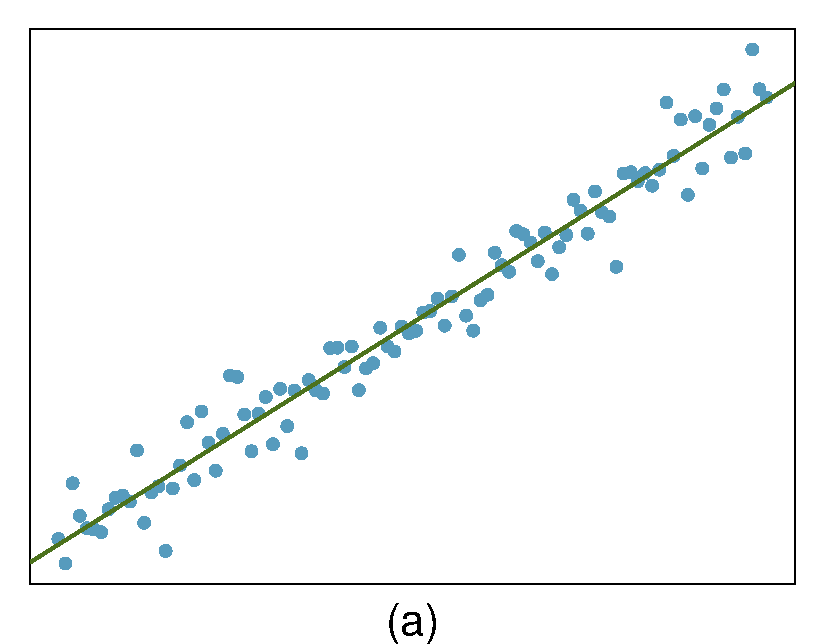
\includegraphics[width=0.42\textwidth]{ch_regr_simple_linear/figures/eoce/visualize_residuals/visualize_residuals_linear.pdf} 
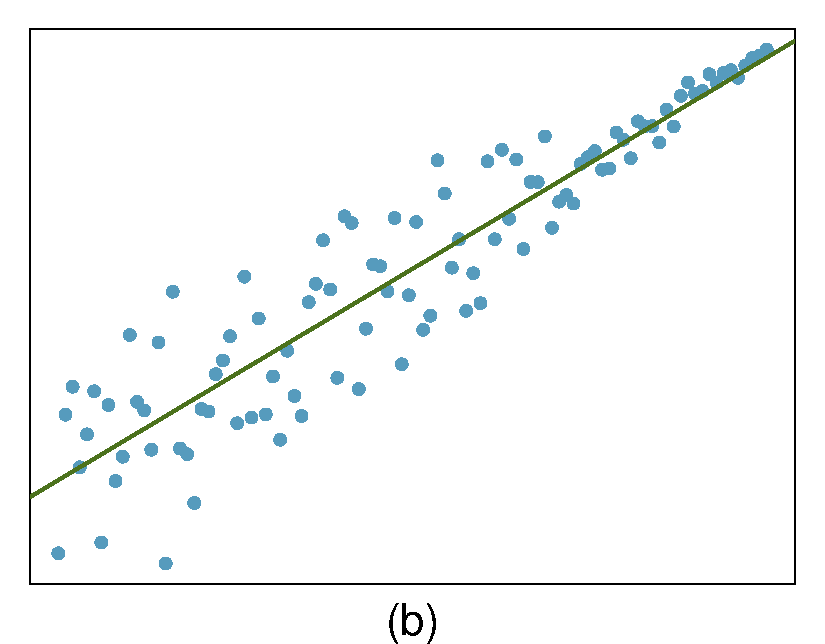
\includegraphics[width=0.42\textwidth]{ch_regr_simple_linear/figures/eoce/visualize_residuals/visualize_residuals_fan_back.pdf}
\end{center}
}{}

% 2

\eoce{\qt{Trends in the residuals\label{trends_in_residuals}} 
Shown below are two plots of residuals 
remaining after fitting a linear model to two different sets of data. 
Describe important features and determine if a linear model would be 
appropriate for these data. Explain your reasoning.
\begin{center}
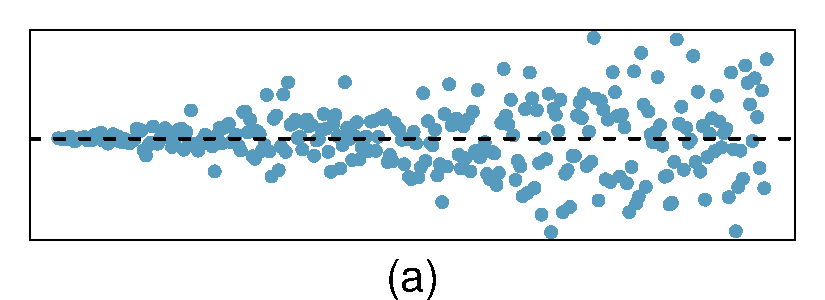
\includegraphics[width=0.42\textwidth]{ch_regr_simple_linear/figures/eoce/trends_in_residuals/trends_in_residuals_fan.pdf} 
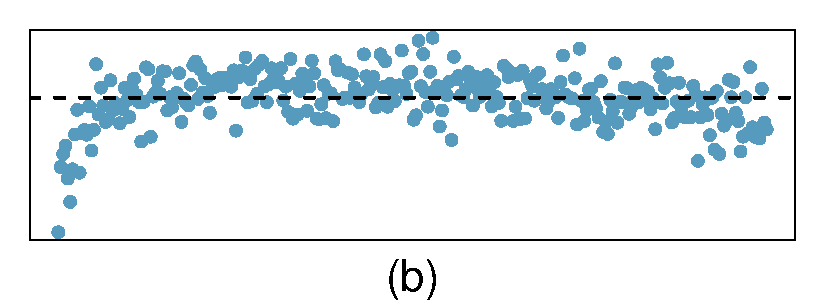
\includegraphics[width=0.42\textwidth]{ch_regr_simple_linear/figures/eoce/trends_in_residuals/trends_in_residuals_log.pdf}
\end{center}
}{}

% 3

\eoce{\qt{Identify relationships, Part I\label{identify_relationships_1}} 
For each of the six plots, 
identify the strength of the relationship (e.g. weak, moderate, or 
strong) in the data and whether fitting a linear model would be 
reasonable.
\begin{center}
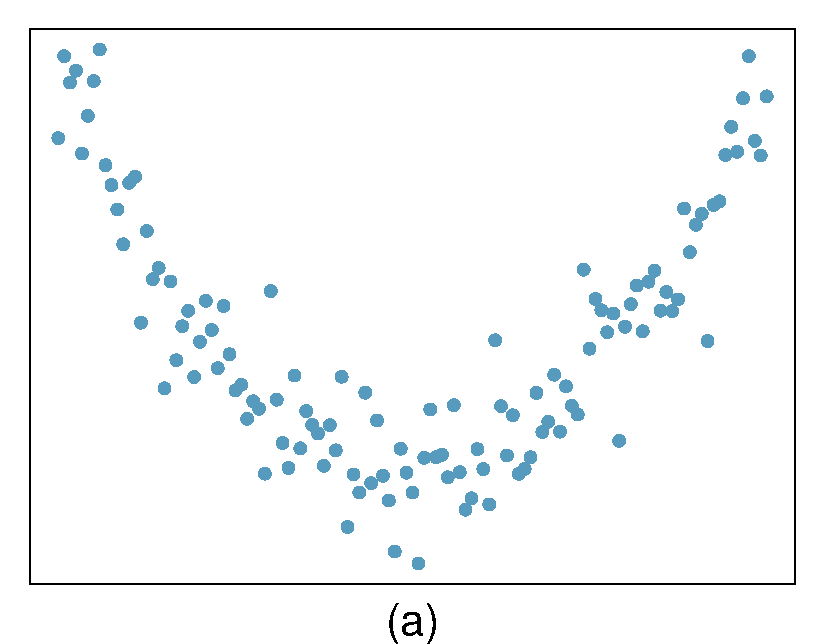
\includegraphics[width=0.32\textwidth]{ch_regr_simple_linear/figures/eoce/identify_relationships_1/identify_relationships_u.pdf}
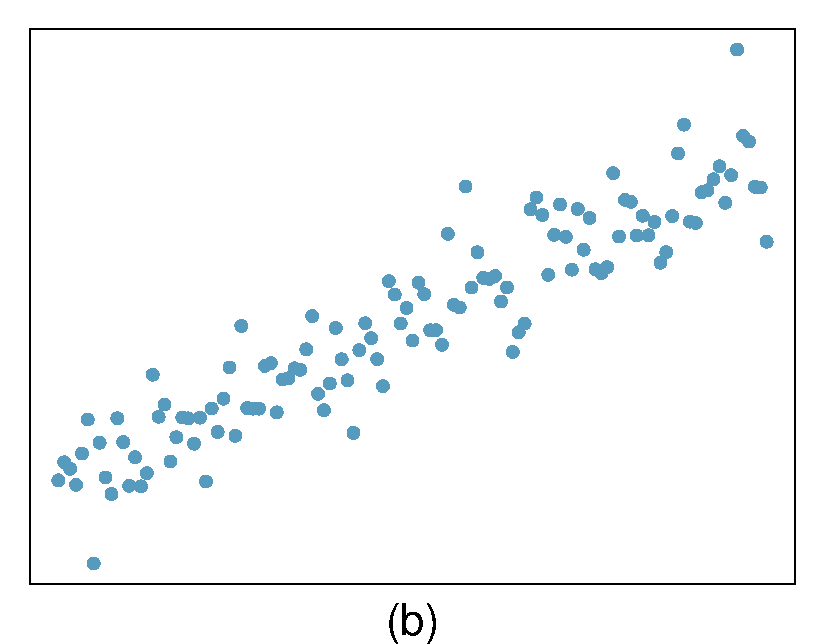
\includegraphics[width=0.32\textwidth]{ch_regr_simple_linear/figures/eoce/identify_relationships_1/identify_relationships_lin_pos_strong.pdf}
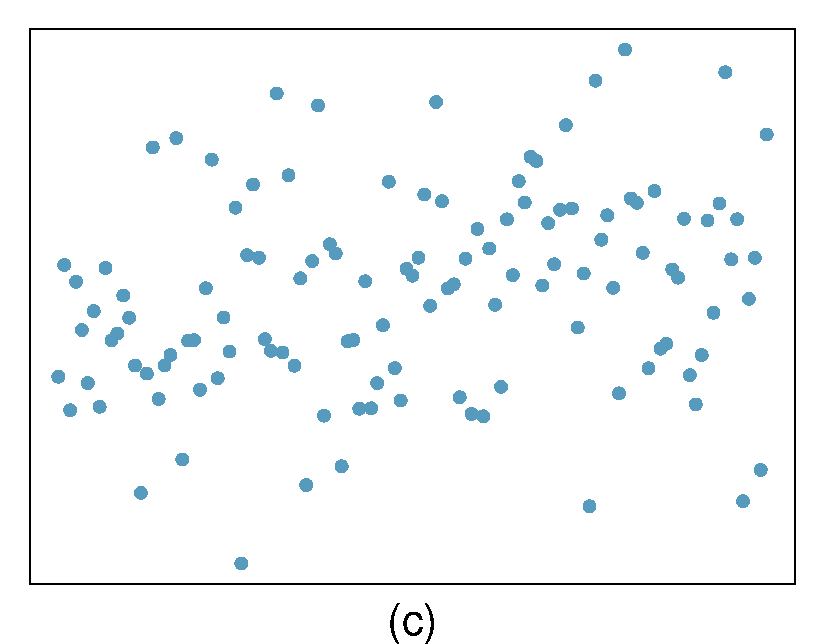
\includegraphics[width=0.32\textwidth]{ch_regr_simple_linear/figures/eoce/identify_relationships_1/identify_relationships_lin_pos_weak.pdf}
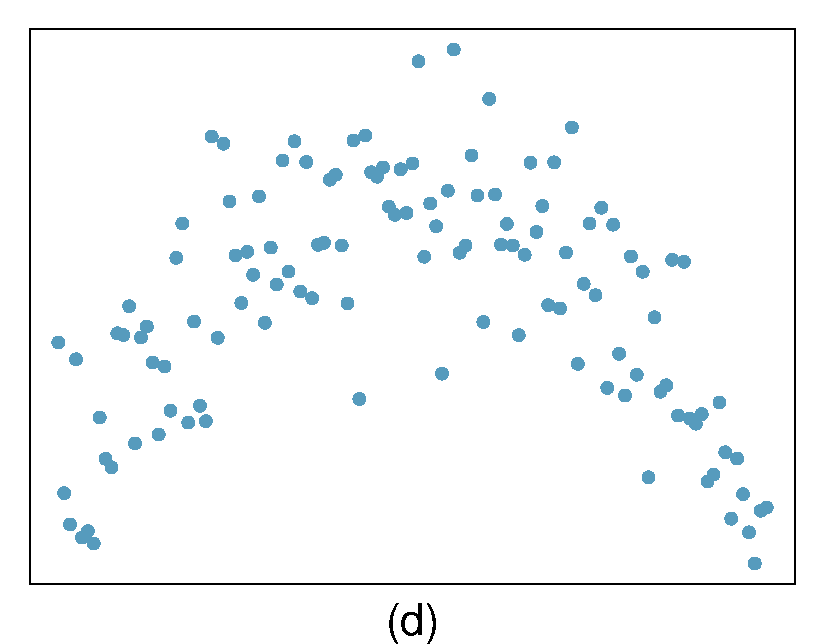
\includegraphics[width=0.32\textwidth]{ch_regr_simple_linear/figures/eoce/identify_relationships_1/identify_relationships_n.pdf}
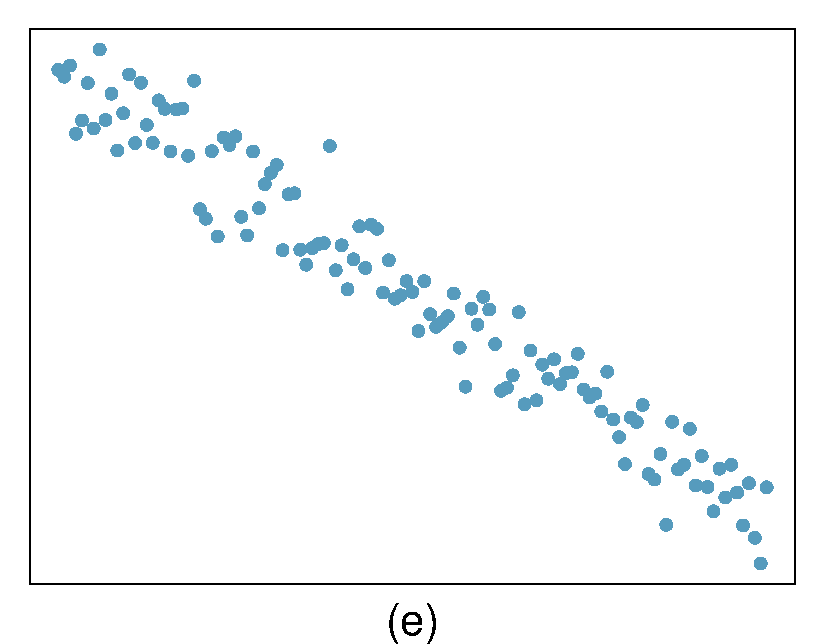
\includegraphics[width=0.32\textwidth]{ch_regr_simple_linear/figures/eoce/identify_relationships_1/identify_relationships_lin_neg_strong.pdf}
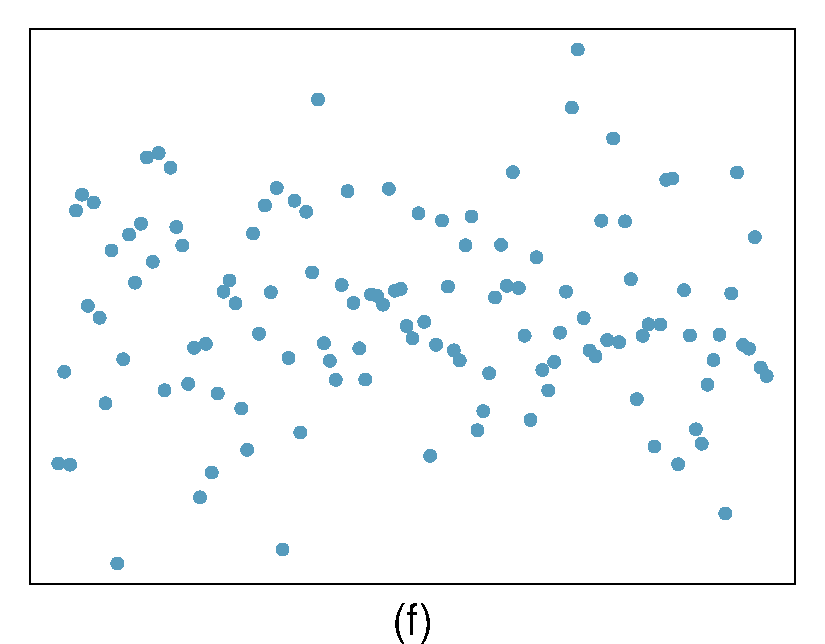
\includegraphics[width=0.32\textwidth]{ch_regr_simple_linear/figures/eoce/identify_relationships_1/identify_relationships_none.pdf}
\end{center}
}{}

% 4

\eoce{\qt{Identify relationships, Part II\label{identify_relationships_2}} 
For each of the six plots, 
identify the strength of the relationship (e.g. weak, moderate, or 
strong) in the data and whether fitting a linear model would be 
reasonable.
\begin{center}
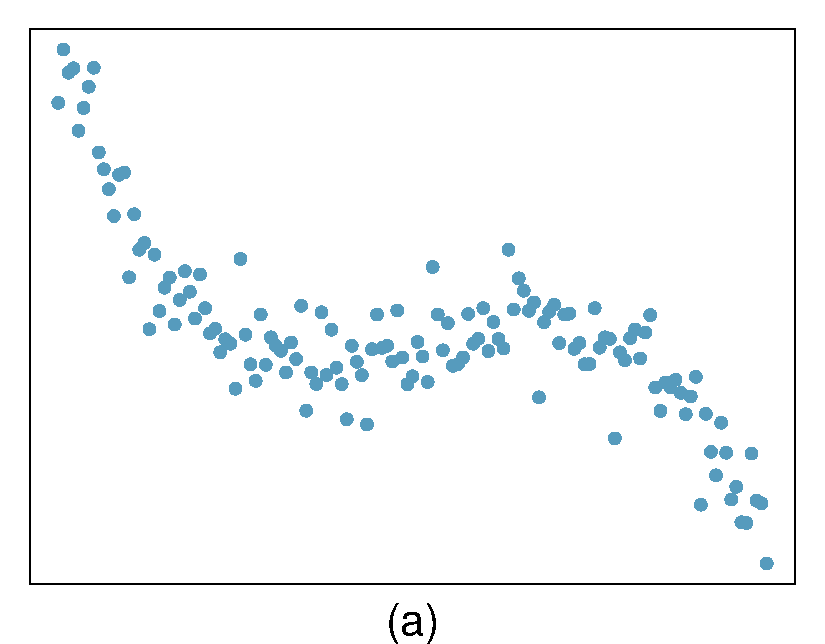
\includegraphics[width=0.32\textwidth]{ch_regr_simple_linear/figures/eoce/identify_relationships_2/identify_relationships_s.pdf}
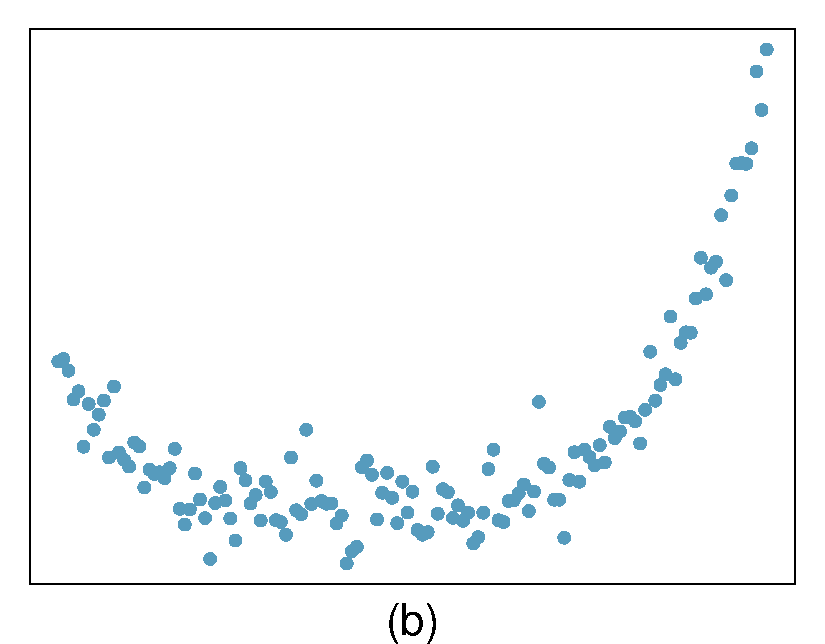
\includegraphics[width=0.32\textwidth]{ch_regr_simple_linear/figures/eoce/identify_relationships_2/identify_relationships_hockey_stick.pdf}
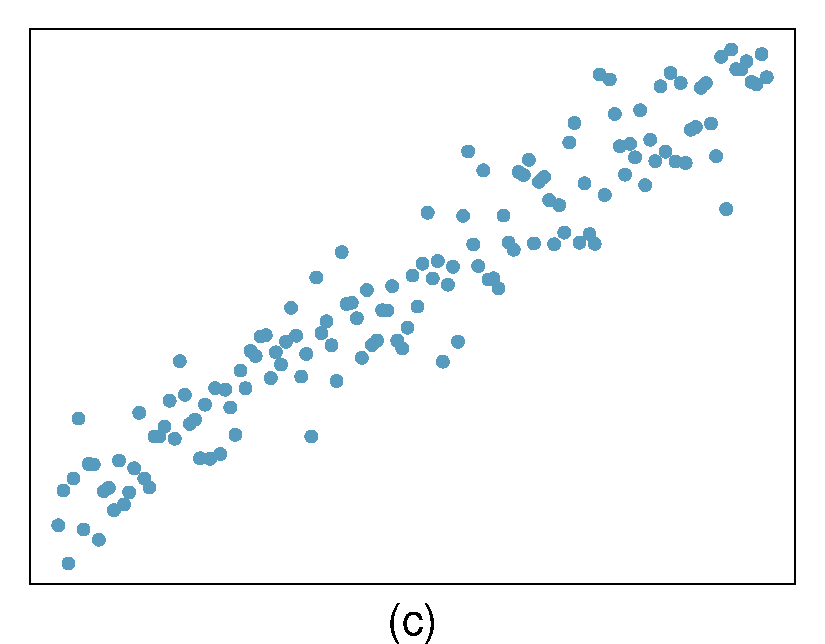
\includegraphics[width=0.32\textwidth]{ch_regr_simple_linear/figures/eoce/identify_relationships_2/identify_relationships_pos_lin_strong.pdf}
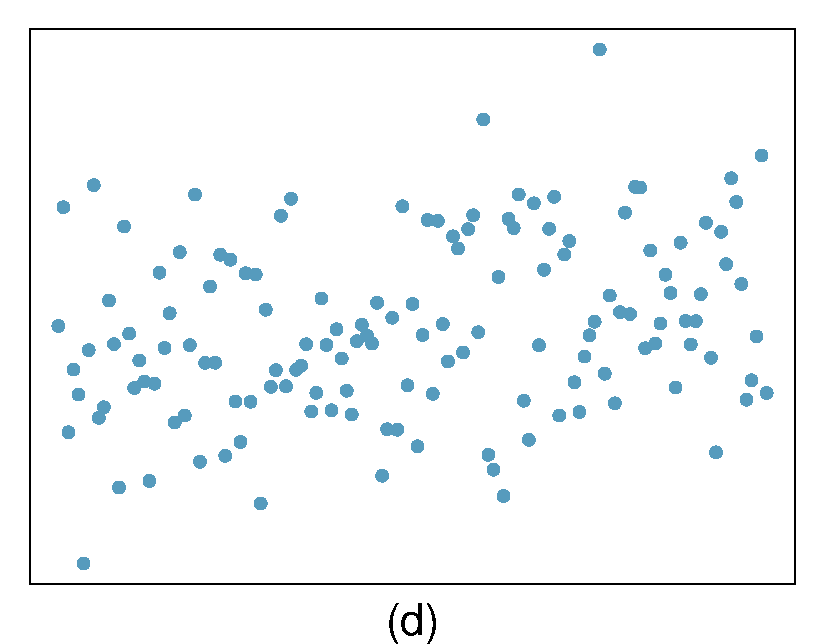
\includegraphics[width=0.32\textwidth]{ch_regr_simple_linear/figures/eoce/identify_relationships_2/identify_relationships_pos_weak.pdf}
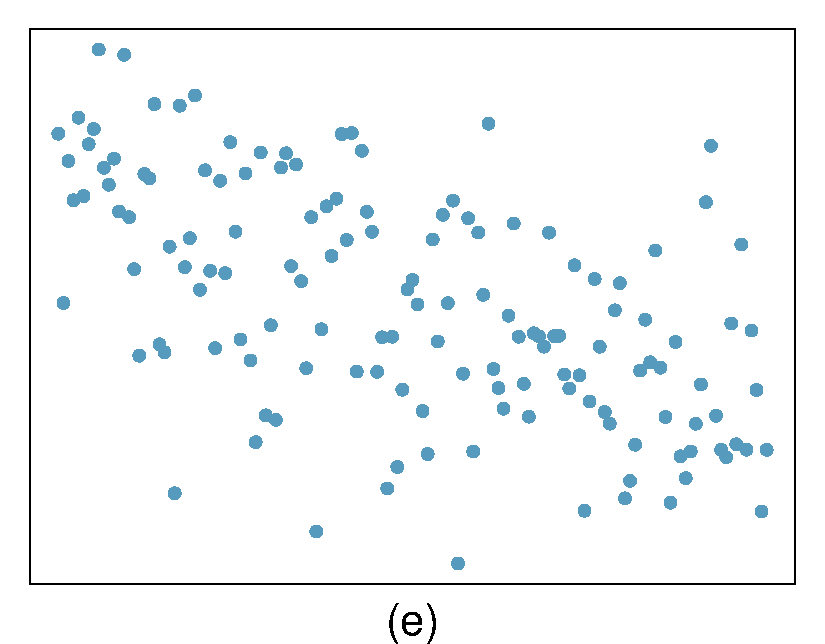
\includegraphics[width=0.32\textwidth]{ch_regr_simple_linear/figures/eoce/identify_relationships_2/identify_relationships_pos_weaker.pdf}
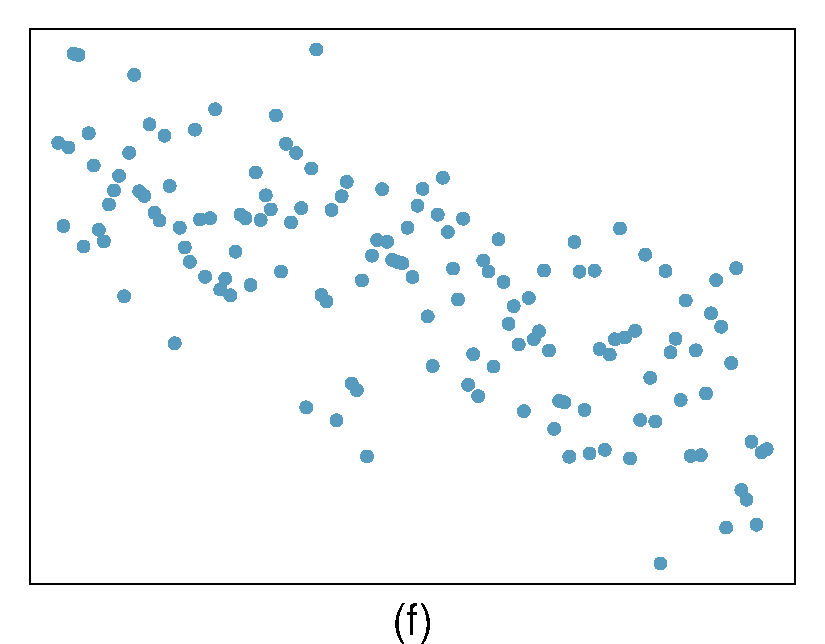
\includegraphics[width=0.32\textwidth]{ch_regr_simple_linear/figures/eoce/identify_relationships_2/identify_relationships_neg_lin_weak.pdf}
\end{center}
}{}

% 5

\eoce{\qt{Exams and grades\label{exams_grades_correlation}} 
The two scatterplots below show the 
relationship between final and mid-semester exam grades recorded 
during several years for a Statistics course at a university.
\begin{parts}
\item Based on these graphs, which of the two exams has the strongest 
correlation with the final exam grade? Explain.
\item Can you think of a reason why the correlation between the exam 
you chose in part (a) and the final exam is higher?
\end{parts}
\begin{center}
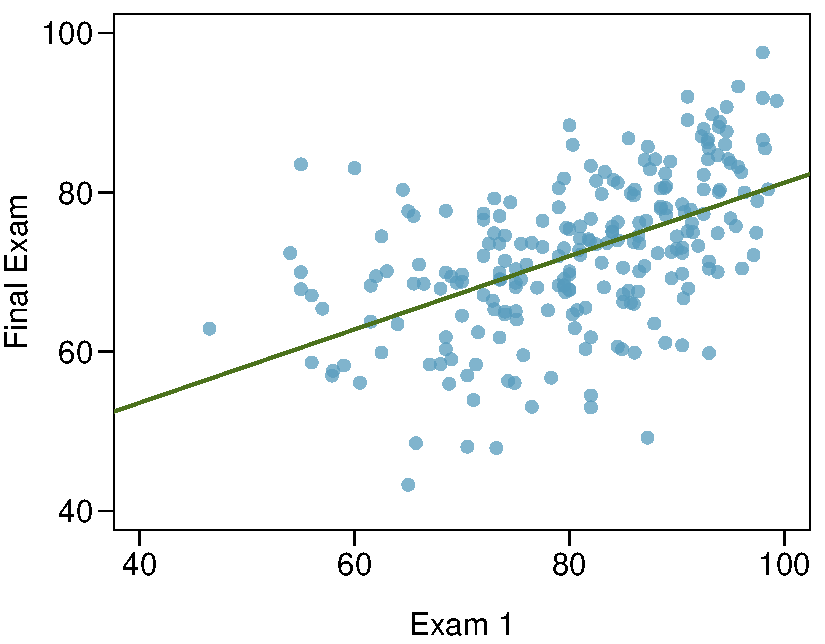
\includegraphics[width=0.485\textwidth]{ch_regr_simple_linear/figures/eoce/exams_grades_correlation/exam_grades_1.pdf}
\hspace{0.02\textwidth}%
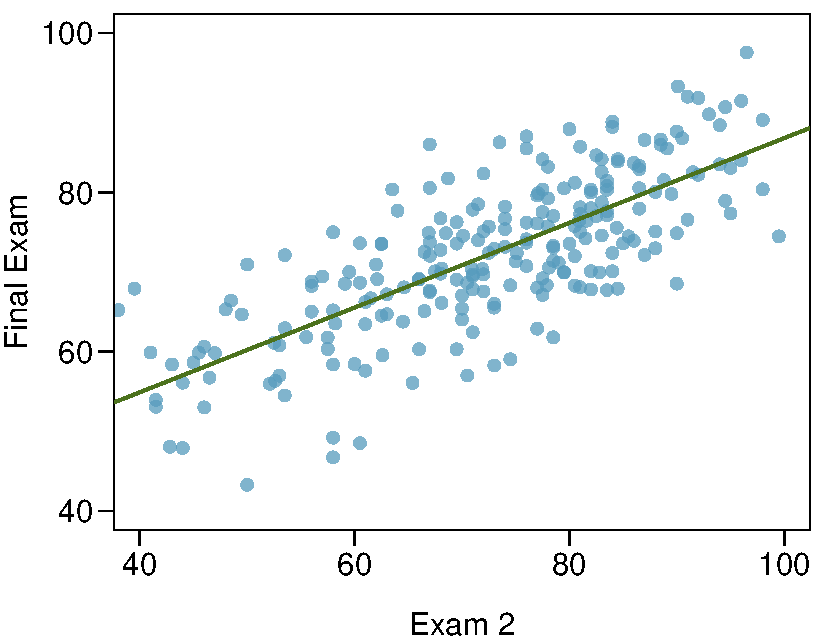
\includegraphics[width=0.485\textwidth]{ch_regr_simple_linear/figures/eoce/exams_grades_correlation/exam_grades_2.pdf}
\end{center}
}{}

% 6

\eoce{\qt{Husbands and wives, Part I\label{husbands_wives_correlation}}
The Great Britain Office of Population Census and Surveys once 
collected data on a random sample of 170 married couples in 
Britain, recording the age (in years) and heights (converted 
here to inches) of the husbands and wives.\footfullcite{Hand:1994} 
The scatterplot on the left shows the wife's age plotted against her 
husband's age, and the plot on the right shows wife's height 
plotted against husband's height.
\newpage
\begin{center}
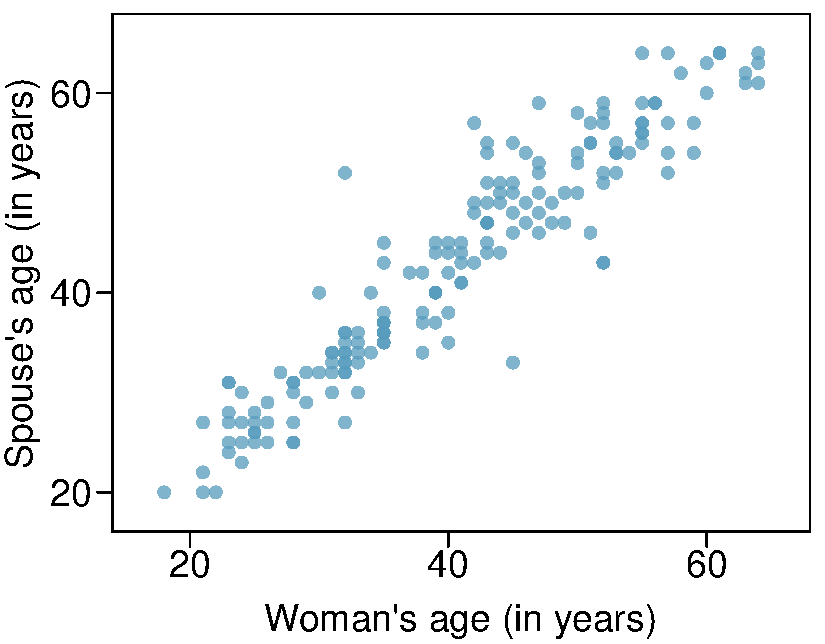
\includegraphics[width=0.38\textwidth]{ch_regr_simple_linear/figures/eoce/husbands_wives_correlation/husbands_wives_age.pdf} 
\hspace{5mm}
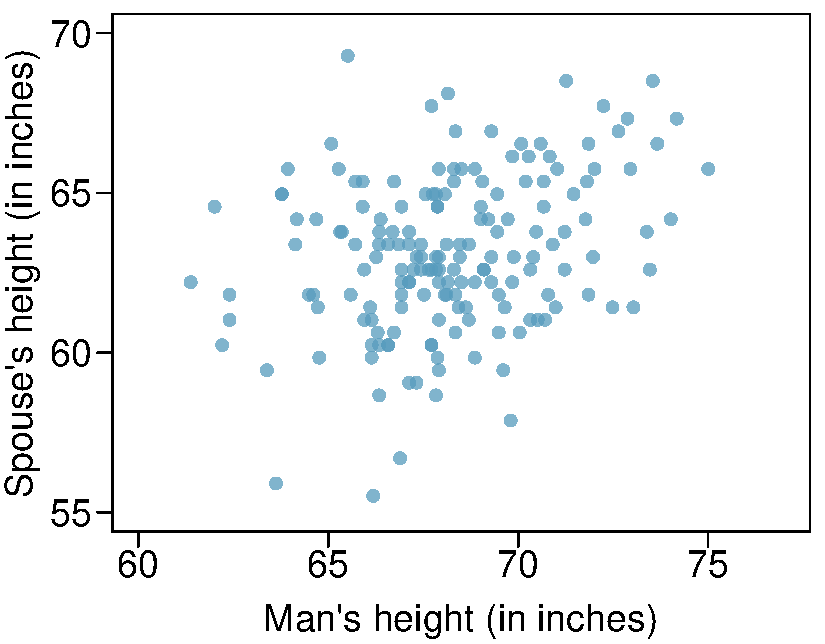
\includegraphics[width=0.38\textwidth]{ch_regr_simple_linear/figures/eoce/husbands_wives_correlation/husbands_wives_height.pdf}
\end{center}
\begin{parts}
\item Describe the relationship between husbands' and wives' ages.
\item Describe the relationship between husbands' and wives' heights.
\item Which plot shows a stronger correlation? Explain your reasoning.
\item Data on heights were originally collected in centimeters, and 
then converted to inches. Does this conversion affect the correlation 
between husbands' and wives' heights?
\end{parts}
}{}

% 7

\eoce{\qt{Match the correlation, Part I\label{match_corr_1}} 
Match each correlation to the corresponding scatterplot.

\noindent%
\begin{minipage}[c]{0.17\textwidth}
\begin{parts}
\item $r = -0.7$
\item $r = 0.45$ 
\item $r = 0.06$
\item $r = 0.92$
\end{parts}\vspace{3mm}
\end{minipage}%
\begin{minipage}[c]{0.83\textwidth}
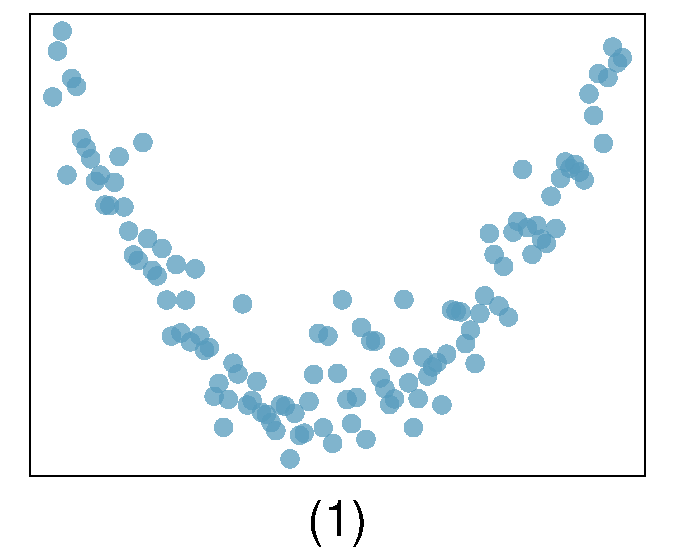
\includegraphics[width=0.245\textwidth]{ch_regr_simple_linear/figures/eoce/match_corr_1/match_corr_1_u}
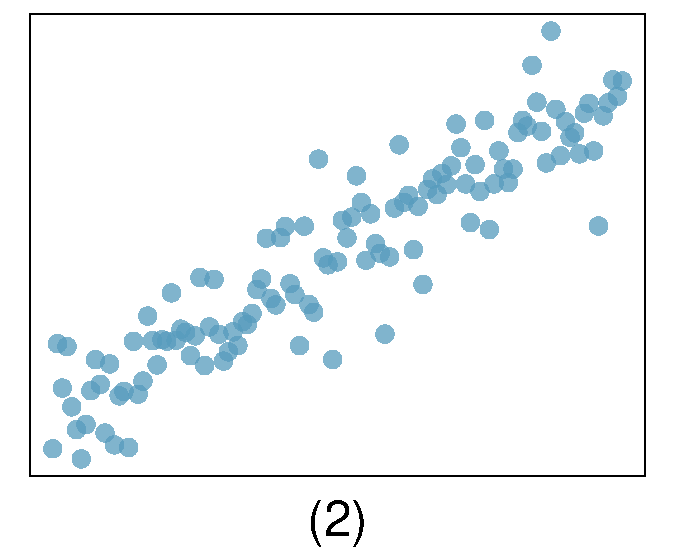
\includegraphics[width=0.245\textwidth]{ch_regr_simple_linear/figures/eoce/match_corr_1/match_corr_2_strong_pos}
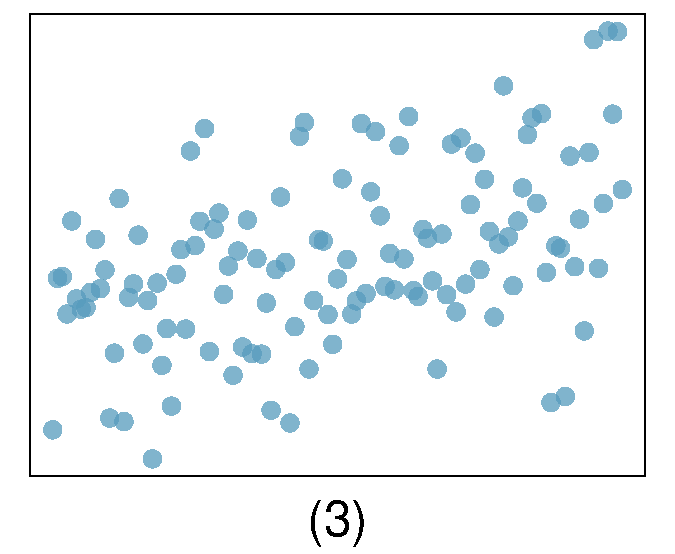
\includegraphics[width=0.245\textwidth]{ch_regr_simple_linear/figures/eoce/match_corr_1/match_corr_3_weak_pos}
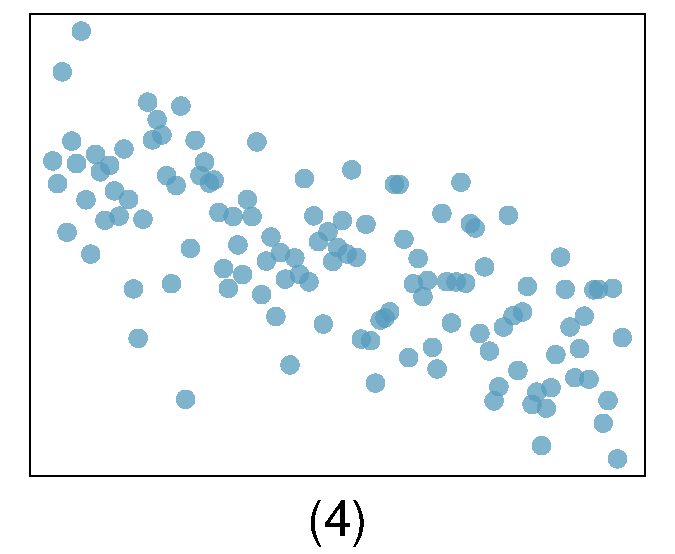
\includegraphics[width=0.245\textwidth]{ch_regr_simple_linear/figures/eoce/match_corr_1/match_corr_4_weak_neg}
\end{minipage}
}{}

% 8

\eoce{\qt{Match the correlation, Part II\label{match_corr_2}} 
Match each correlation to the corresponding scatterplot.

\noindent%
\begin{minipage}[c]{0.17\textwidth}
\begin{parts}
\item $r = 0.49$
\item $r = -0.48$ 
\item $r = -0.03$ 
\item $r = -0.85$
\end{parts}\vspace{3mm}
\end{minipage}%
\begin{minipage}[c]{0.83\textwidth}
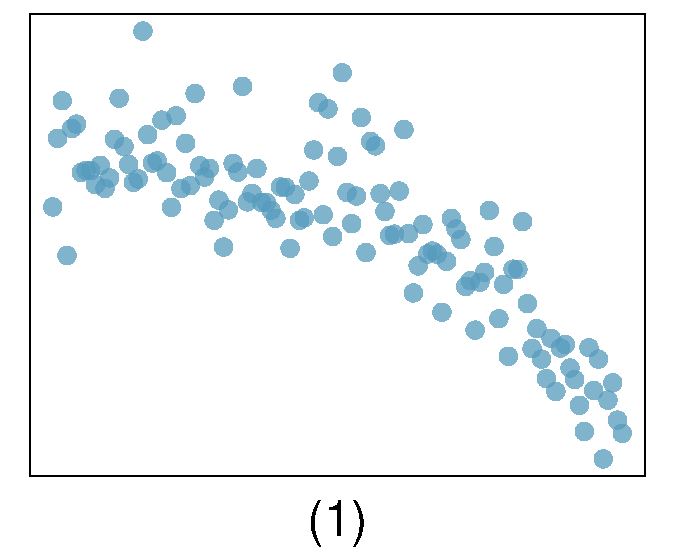
\includegraphics[width=0.245\textwidth]{ch_regr_simple_linear/figures/eoce/match_corr_2/match_corr_1_strong_neg_curved}
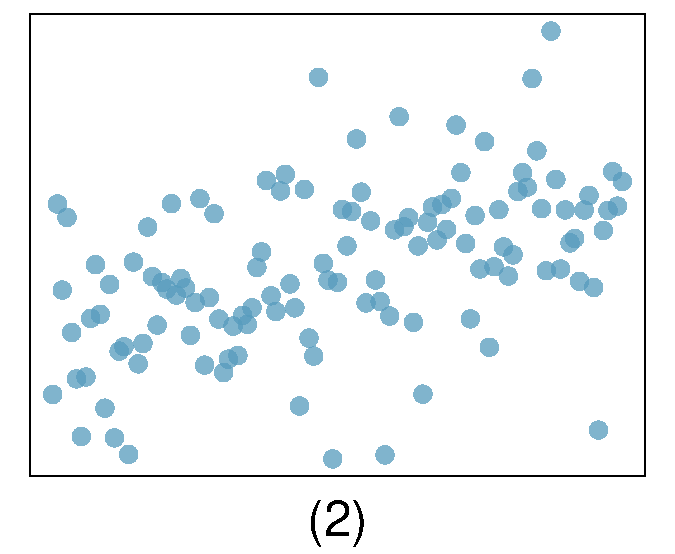
\includegraphics[width=0.245\textwidth]{ch_regr_simple_linear/figures/eoce/match_corr_2/match_corr_2_weak_pos}
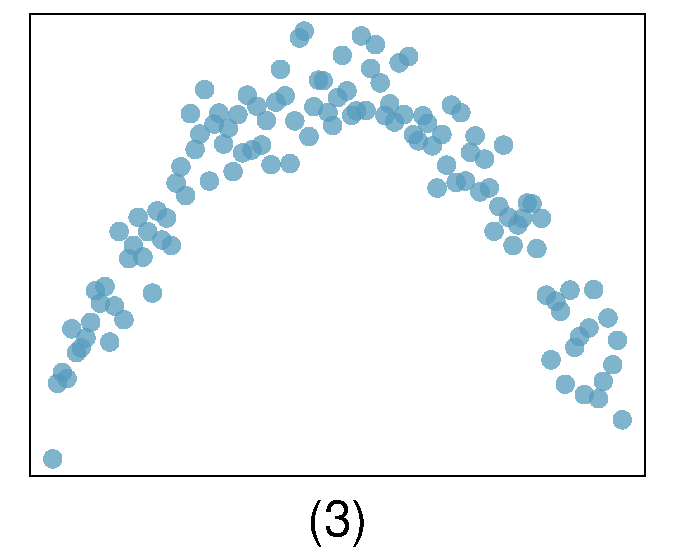
\includegraphics[width=0.245\textwidth]{ch_regr_simple_linear/figures/eoce/match_corr_2/match_corr_3_n}
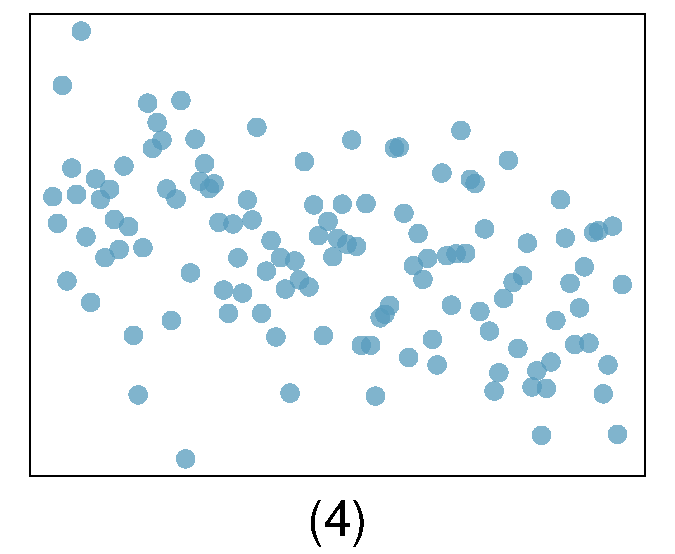
\includegraphics[width=0.245\textwidth]{ch_regr_simple_linear/figures/eoce/match_corr_2/match_corr_4_weak_neg}
\end{minipage}
}{}

% 9

\eoce{\qt{Speed and height\label{speed_height_gender}} 1,302 UCLA students 
were asked to fill out a survey where they were asked about their height, 
fastest speed they have ever driven, and gender. The scatterplot on the 
left displays the relationship between height and fastest speed, and 
the scatterplot on the right displays the breakdown by gender in 
this relationship.
\begin{center}
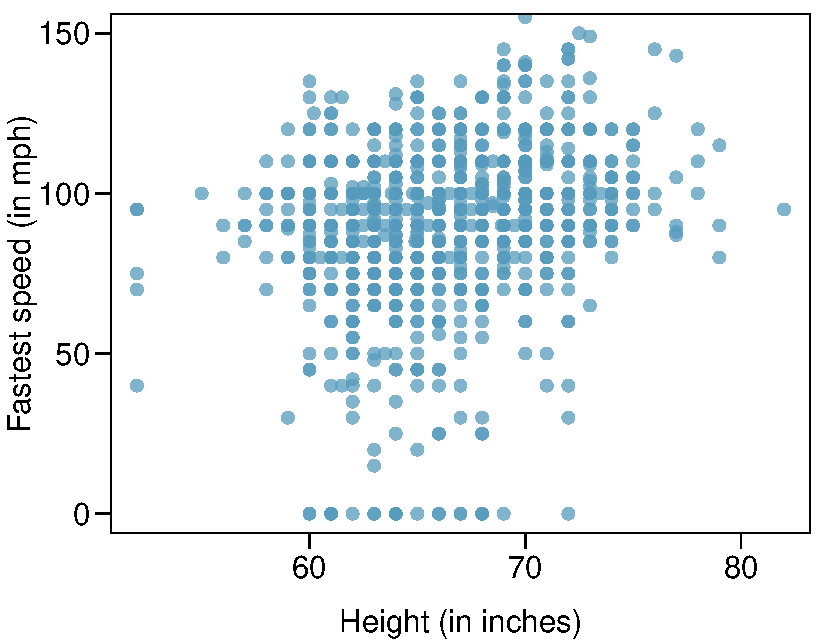
\includegraphics[width=0.485\textwidth]{ch_regr_simple_linear/figures/eoce/speed_height_gender/speed_height.pdf}
\hspace{0.02\textwidth}%
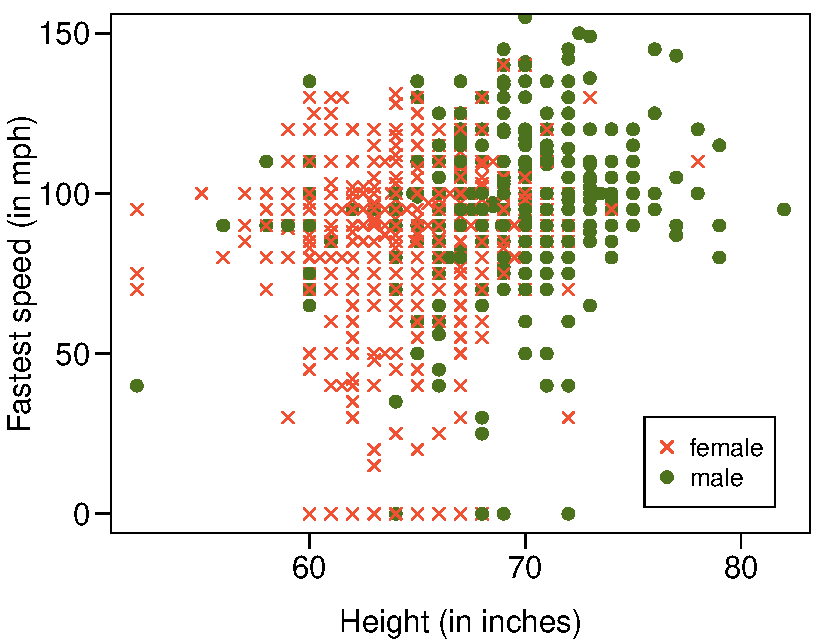
\includegraphics[width=0.485\textwidth]{ch_regr_simple_linear/figures/eoce/speed_height_gender/speed_height_gender.pdf}
\end{center}
\begin{parts}
\item Describe the relationship between height and fastest speed.
\item Why do you think these variables are positively associated?
\item What role does gender play in the relationship between height 
and fastest driving speed?
\end{parts}
}{}

% 10

\eoce{\qt{Guess the correlation\label{guess_correlation}} Eduardo and Rosie 
are both collecting data on number of rainy days in a year and the total 
rainfall for the year. Eduardo records rainfall in inches and Rosie in 
centimeters. How will their correlation coefficients compare?
}{}

% 11

\eoce{\qt{The Coast Starlight, Part I\label{coast_starlight_corr_units}} 
The Coast Starlight Amtrak train runs from Seattle to Los Angeles. 
The scatterplot below displays the distance between each stop 
(in miles) and the amount of time it takes to travel from one stop 
to another (in minutes).\vspace{2mm}

\noindent\begin{minipage}[c]{0.4\textwidth}
{\raggedright\begin{parts}
\item Describe the relationship between distance and travel time.
\item How would the relationship change if travel time was instead measured 
in hours, and distance was instead measured in kilometers?
\item Correlation between travel time (in miles) and distance (in minutes) 
is $r = 0.636$. What is the correlation between travel time (in kilometers) 
and distance (in hours)?
\end{parts}\vspace{7mm}}
\end{minipage}
\begin{minipage}[c]{0.1\textwidth}
$\:$\\
\end{minipage}
\begin{minipage}[c]{0.485\textwidth}
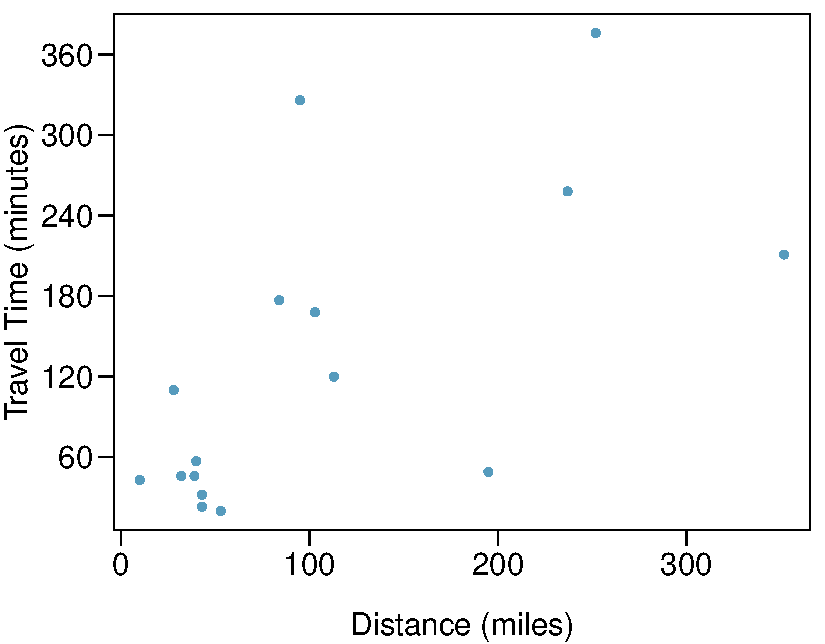
\includegraphics[width=\textwidth]{ch_regr_simple_linear/figures/eoce/coast_starlight_corr_units/coast_starlight.pdf}
\end{minipage}
}{}

% 12

\eoce{\qt{Crawling babies, Part I\label{crawling_babies_corr_units}}  
A study conducted at the University of Denver investigated whether babies 
take longer to learn to crawl in cold months, when they are often bundled 
in clothes that restrict their movement, than in warmer months.
\footfullcite{Benson:1993} Infants born during the study year were split 
into twelve groups, one for each birth month. We consider the average 
crawling age of babies in each group against the average temperature when 
the babies are six months old (that's when babies often begin trying to 
crawl). Temperature is measured in degrees Fahrenheit (\degree F) and age 
is measured in weeks.\vspace{2mm}

\noindent\begin{minipage}[c]{0.4\textwidth}
{\raggedright\begin{parts}
\item Describe the relationship between temperature and crawling age.
\item How would the relationship change if temperature was measured in 
degrees Celsius (\degree C) and age was measured in months?
\item The correlation between temperature in \degree F and age in weeks 
was $r=-0.70$. If we converted the temperature to \degree C and age to 
months, what would the correlation be?
\end{parts}\vspace{3mm}}
\end{minipage}
\begin{minipage}[c]{0.1\textwidth}
$\:$\\
\end{minipage}
\begin{minipage}[c]{0.485\textwidth}
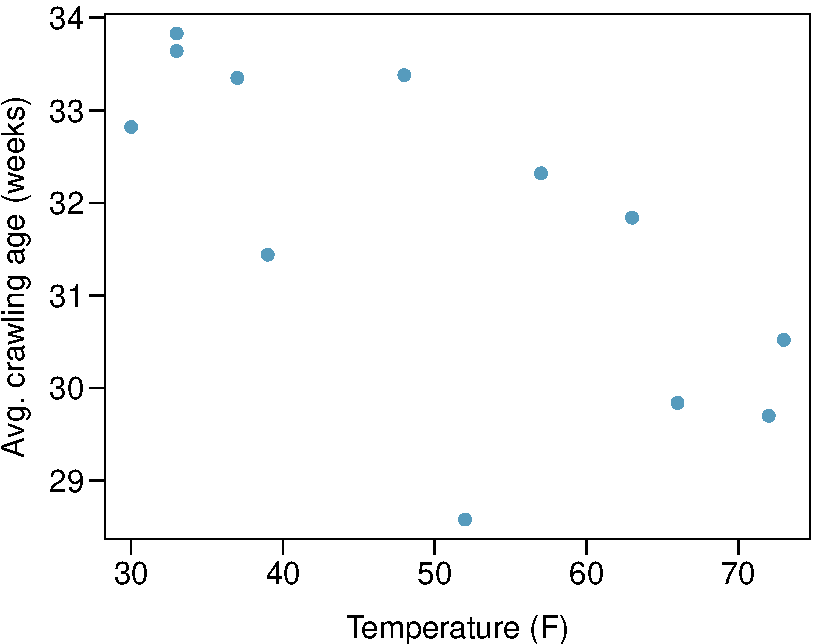
\includegraphics[width=\textwidth]{ch_regr_simple_linear/figures/eoce/crawling_babies_corr_units/crawling_babies.pdf}
\end{minipage}
}{}

% 13

\eoce{\qt{Body measurements, Part I\label{body_measurements_shoulder_height_corr_units}} 
Researchers studying anthropometry collected body girth measurements and 
skeletal diameter measurements, as well as age, weight, height and gender 
for 507 physically active individuals.\footfullcite{Heinz:2003} The 
scatterplot below shows the relationship between height and shoulder 
girth (over deltoid muscles), both measured in centimeters.\vspace{3mm}

\noindent%
\begin{minipage}[c]{0.4\textwidth}
{\raggedright\begin{parts}
\item Describe the relationship between shoulder girth and height.
\item How would the relationship change if shoulder girth was measured 
in inches while the units of height remained in centimeters?
\end{parts}\vspace{20mm}}
\end{minipage}
\begin{minipage}[c]{0.1\textwidth}                  
$\:$\\
\end{minipage}
\begin{minipage}[c]{0.485\textwidth}
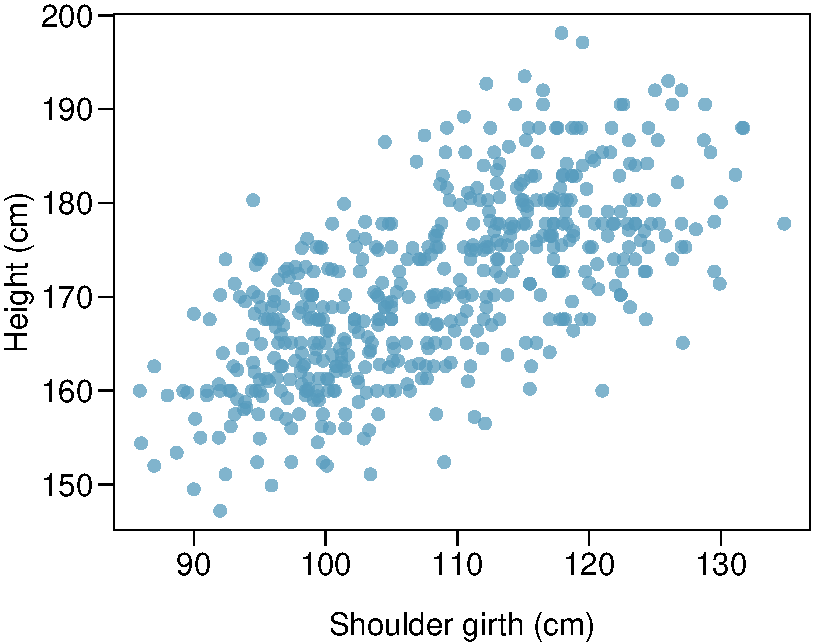
\includegraphics[width=\textwidth]{ch_regr_simple_linear/figures/eoce/body_measurements_shoulder_height_corr_units/body_measurements_height_shoulder_girth.pdf}
\end{minipage}
}{}

% 14

\eoce{\qt{Body measurements, Part II\label{body_measurements_hip_weight_corr_units}} 
The scatterplot below shows the relationship between weight 
measured in kilograms and hip girth measured in centimeters 
from the data described in 
Exercise~\ref{body_measurements_shoulder_height_corr_units}.%
\vspace{3mm}

\noindent%
\begin{minipage}[c]{0.4\textwidth}
{\raggedright\begin{parts}
\item Describe the relationship between hip girth and weight.
\item How would the relationship change if weight was measured in pounds 
while the units for hip girth remained in centimeters?
\end{parts}\vspace{20mm}}
\end{minipage}
\begin{minipage}[c]{0.1\textwidth}
$\:$\\
\end{minipage}
\begin{minipage}[c]{0.485\textwidth}
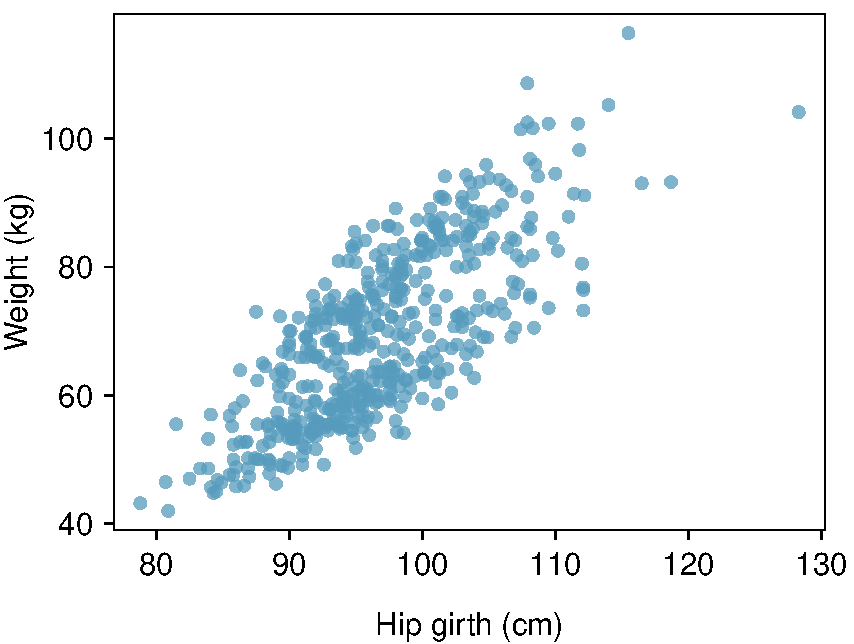
\includegraphics[width=\textwidth]{ch_regr_simple_linear/figures/eoce/body_measurements_hip_weight_corr_units/body_measurements_weight_hip_girth.pdf}
\end{minipage}
}{}

% 15

\eoce{\qt{Correlation, Part I\label{corr_husband_wife_age}} \videohref{ahss_eoce_sol-corr_husband_wife_age}\ \ What would be the 
correlation between the ages of husbands and wives if men always married 
woman who were
\begin{parts}
\item 3 years younger than themselves? 
\item 2 years older than themselves? 
\item half as old as themselves?
\end{parts}
}{}

% 16

\eoce{\qt{Correlation, Part II\label{corr_men_women_salary}} What would be the 
correlation between the annual salaries of males and females at a company 
if for a certain type of position men always made
\begin{parts}
\item \$5,000 more than women?
\item 25\% more than women?
\item 15\% less than women?
\end{parts}
}{}
